\documentclass{article}
\usepackage{tikz}
\usetikzlibrary{angles, quotes}
\usepackage{amssymb}
\usepackage{pgfplots}
\pgfplotsset{width=10cm,compat=1.9}
\usepgfplotslibrary{statistics}
\usepackage[left=2.54cm,right=2.54cm,top=2.54cm,bottom=2.54cm]{geometry}
\usepackage{tasks} %Paquete necesario para la producción de items horizontales para algunos ejercicios de tarea empleando el comando /begin{multicols}}{#}.../end{multicols} para ayudarnos a reducir las páginas
\usepackage{pdflscape} %comando que permite cambiar a orientación horizontal las hojas%
\usepackage{soul} %Paquete para permitir la compilación de acentos usando el comando {\hl{}}}\\
\sethlcolor{yellow(munsell)} %comando para definir el color para el subrayado usando el comando \hl
\usepackage[utf8]{inputenc}
\usepackage[spanish]{babel}
\usepackage{icomma}
\usepackage{ragged2e}
\usepackage{siunitx}
\usepackage{url}
\usepackage[colorlinks=true, urlcolor=blue,  linkcolor=black, citecolor=green]{hyperref}
\usepackage{pdfpages}
\usepackage{blindtext} %Paquete que genera texto ficticio (dummy text) con el comando: \blindtext
\usepackage{cancel} %in the preamble gives you four different modes of striking through: \cancel{text to cancel} draws a diagonal line (slash) through its argument, \bcancel{text to cancel} uses the negative slope (a backslash), \xcancel{text to cancel} draws an X (actually \cancel plus \bcancel), \cancelto{〈value〉}{〈expression〉} draws a diagonal arrow through the 〈expression〉pointing to the 〈value〉 (math-mode only)
\usepackage{csquotes}
\usepackage{afterpage}
\usepackage{parskip} 
\usepackage{float}
\usepackage{enumitem}
\usepackage{multicol}%Paquete que permite la creación aislada de columnas de texto. De esta forma se reduce la cantidad de páginas en nuestro documento
\usepackage{lipsum} %Paquete que genera texto de relleno al igual que \usepackage{blindtext}, se usa con el comando \lipsum[#-#] los #(hashtags) delimitan el número de páginas que deseamos ocupar del paquete lipsum para usarlos como relleno. 

% Definir el comando personalizado para la nota
\newcommand{\mynote}[1]{%
\begin{tikzpicture}[baseline=-0.75ex]
\node[draw, circle, fill=Apple Green!60, inner sep=2pt] (note) {\textbf{Nota:}};
\end{tikzpicture}%
\ \textit{#1}%
}

\newenvironment{Figura}
{\par\medskip\noindent\minipage{\linewidth}}
{\endminipage\par\medskip}
\usepackage{caption}
\usepackage[
backend=biber,
sorting=none,
url=true
]{biblatex} %bibliografía
\addbibresource{biblio.bib}
% Establecer el espacio entre las entradas de la bibliografía
\setlength{\bibitemsep}{1\baselineskip} % Puedes ajustar el valor según tus preferencias
\usepackage{amsmath,amsthm,amssymb,amsfonts}
\usepackage{pifont} %Permite la compilación del comando \xmark: es el símbolo de la tachita
\usepackage{mathtools} %permite la compilación de símbolos para matrices
\usepackage{empheq} %Paquete que se relaciona con \usepackage[most]{tcolorbox} para la creación de cuadros/cajas de colores para delimitar los resultados matemáticos o líneas de texto usando la línea de comando: \begin{empheq}[box={\mymath[colback=orange(webcolor)!70,drop lifted shadow]}]{equation*} \end{empheq}
\usepackage[most]{tcolorbox} %Paquete que se relaciona con \usepackage{empheq} para la creación de cuadros/cajas de colores para delimitar los resultados matemáticos o líneas de texto
\renewcommand{\qedsymbol}{$\blacksquare$}
\usetikzlibrary{positioning,decorations.pathreplacing} %Paquete que permite la compilación de llaves para cuadros sinópticos (brace diagram) 
\usepackage{schemata} %The schemata package is designed just for these brace diagrams
\usepackage{booktabs}

\newcommand\AB[2]{\schema{\schemabox{#1}}{\schemabox{#2}}} %comando o paquete necesario para crear cuadros sinópticos

\newtcbox{\mymath}[1][]{%
nobeforeafter, math upper, tcbox raise base,
enhanced, colframe=blue!30!black,
colback=blue!30, boxrule=1pt,
#1} %Comando importante para encasillar los resultados matemáticos en cajas de diferentes colores, se relaciona con los paquetes \usepackage{empheq} y \usepackage[most]{tcolorbox} 

\newenvironment{sysmatrix}[1]
{\left(\begin{array}{@{}#1@{}}}
{\end{array}\right)}
\newcommand{\ro}[1]{%
\xrightarrow{\mathmakebox[\rowidth]{#1}}%
}
\newlength{\rowidth}% row operation width
\AtBeginDocument{\setlength{\rowidth}{3em}}  %Comando importante para laproducción de lineas de operaciones entre matrices, método de Gauss o Gauss Jordan se relaciona con \newenvironment{sysmatrix}

%formato para cambiar el horario a español
\usepackage[spanish]{datetime2}
\DTMsetdatestyle{spanish}

\renewcommand{\today}{\DTMdisplaydate{\the\year}{\the\month}{\the\day }{-1}}
%%%%%%%%%%%%%%%%%%%%%%%%%%%%%%%%%%%%%%%%%

\usepackage{datetime}
\newcommand{\mycurrenttime}{\xxivtime}

%%%%%%%%%%%%%%%%%%%%%%%%%%%%%%%%%%%%%%%%%%%%%%%%%%%%%%%%%%%%%%%%%%%%%%%%%%%%%%%%%%%%%%%%%%%%%%%%%%%%%%%%%%%%%%%%%%%%%%%%%%%%%%%%%%%%%%%%%%%%%%%%%


%%%%%%%%%%%%%Caja de color para el título%%%%%%%%%%%%%%%%%%%%%%%%%%%%%%%%%%%%%%%%%%%%%%%%%%%%%%

\definecolor{myframecolor}{RGB}{1, 45, 75} % Prussian Blue
\definecolor{myboxcolor}{RGB}{0, 107, 92} % Apple Green

\newtcolorbox{mybox}{
enhanced,
colback=myboxcolor!7, % Color de fondo del cuadro
colframe=myframecolor, % Color del marco del cuadro
arc=0pt,
boxrule=1pt,
borderline west={2mm}{-10mm}{myframecolor}, % Borde en el lado izquierdo
sharp corners=southwest,
width=\linewidth,
before=\par\vspace{\bigskipamount}, % Espacio antes del cuadro
after=\par\vspace{\bigskipamount} % Espacio después del cuadro
}


\newcommand{\euler}{e} %Comando para producir letra e de euler
\newenvironment{remark}{\par\vfill\footnotesize % Vertical white space above the remark and smaller font size
\begin{list}{}{
	\leftmargin=80pt % Indentation on the left
	\rightmargin=60pt}\item\ignorespaces % Indentation on the right
\makebox[-2.5pt]{\begin{tikzpicture}[overlay]
		\node[draw=Horizon!60,line width=2.5pt,circle,fill=Horizon!25,font=\sffamily\bfseries,inner sep=4pt,outer sep=0pt] at (-19pt,5pt){\textcolor{Horizon}{Nota}};\end{tikzpicture}} % Blue Nota in a circle
\advance\baselineskip -1pt}{\end{list}\vskip5pt} % Tighter line spacing and white space after remark
\usepackage{graphicx}

\usepackage{titling}

%colores.tex

%colores que podemos usar en el documento


\usepackage{xcolor}


	%%%%%%%%%%%%%%%%%%%%%%%%%%%%%%%%%%%%%%%%%%%%%%%%%%%%%%%%%%%%Gamas de Azul%%%%%%%%%%%%%%%%%%%%%%%%%%%%%%%%%%%%%%%%%%%%%%%%%%%%%%%%%%%%%%%%%%%%%%%%%%%%%%%%%%%%%%%%%%%%%%%%%%%%%%%%%%%%%%%%%%%%%%%%%%%%%%%%%%%%%%%%%%%%%%%%%%%%%%%%%%%%%%%%%%%%%%%
	
	\definecolor{Cerulean}{RGB}{6, 145, 210} %Azul MercadoPago
	\definecolor{prussianblue}{RGB}{1, 45, 75} %Azul de Prusia
	\definecolor{Blue Sapphire}{RGB}{15, 93, 136}  %Azul Blue Sapphire
	\definecolor{Aguamarina}{rgb}{0.5, 1.0, 0.83} %Azul aguamarina
	\definecolor{trueblue}{rgb}{0.0, 0.45, 0.81} %Azul océano
	\definecolor{Tarawera}{RGB}{6, 48, 70} %Azul fuerte
	\definecolor{palatinateblue}{rgb}{0.15, 0.23, 0.89} %Azul palatinado
	\definecolor{Lochmara}{RGB}{9, 116, 189}  %Azul océano fuerte
	\definecolor{Green vogue}{RGB}{4, 40, 85}  %Azul tenue fuerte
	\definecolor{Horizon}{RGB}{88, 132, 169} % Celeste-cielo fuerte
	\definecolor{blizzardblue}{rgb}{0.67, 0.9, 0.93} %Celeste
	\definecolor{Hippie Blue}{RGB}{92, 148, 179}  %Celeste pastel
	\definecolor{Victoria}{RGB}{67, 68, 140}  %Victoria
	\definecolor{Logan}{RGB}{164, 168, 204}  %Logan
	
	%%%%%%%%%%%%%%%%%%%%%%%%%%%%%%%%%%%%%%%%%%%%%%%%%%%%%%%%%%%%Gamas de Verde%%%%%%%%%%%%%%%%%%%%%%%%%%%%%%%%%%%%%%%%%%%%%%%%%%%%%%%%%%%%%%%%%%%%%%%%%%%%%%%%%%%%%%%%%%%%%%%%%%%%%%%%%%%%%%%%%%%%%%%%%%%%%%%%%%%%%%%%%%%%%%%%%%%%%%%%%%%%%%%%%%%%%%
	
	\definecolor{Surfie Green}{RGB}{12, 131, 123} %Verde Klar
	\definecolor{Bottle Green}{RGB}{8, 52, 28} %Verde alga
	\definecolor{Apple Green}{RGB}{125, 191, 3} %Verde Manzana
	\definecolor{Android Green}{RGB}{156, 196, 61} %Verde Android Green
	\definecolor{Viridian Green}{RGB}{15, 151, 160} % Verde Viridian Green
	\definecolor{tealgreen}{rgb}{0.0, 0.51, 0.5} %Verde Azulado, azul cerceta
	\definecolor{pakistangreen}{rgb}{0.0, 0.4, 0.0} %Verde Pakistán 
	\definecolor{Bluechill}{RGB}{11, 150, 144} %Verde-azulado suave
	\definecolor{Lochinvar}{RGB}{36, 142, 137} %Verde pálido
	\definecolor{Lemon Ginger}{RGB}{170, 164, 40} %Verde lima
	\definecolor{Earls Green}{RGB}{177, 196, 56} %verde claro-manzana
	\definecolor{Saratoga}{RGB}{85, 100, 19}  %Verde-ciénaga  pantano (lodo)
	\definecolor{Deep Sea Green}{RGB}{8, 83, 94} %Verde-azulado tenue oscuro
	\definecolor{tropicalrainforest}{rgb}{0.0, 0.46, 0.37} %Verde Cyan tono oscuro
	\definecolor{brightturquoise}{RGB}{1, 196, 254} %Turquesa Brillante
	\definecolor{Medium Aquamarine}{RGB}{116, 204, 159} %Agua marina
	\definecolor{Elephant}{RGB}{16, 52, 60} %Azul de shell de vi
	
	
	%%%%%%%%%%%%%%%%%%%%%%%%%%%%%%%%%%%%%%%%%%%%%%%%%%%%%%%%%%%%Gamas de Amarillo%%%%%%%%%%%%%%%%%%%%%%%%%%%%%%%%%%%%%%%%%%%%%%%%%%%%%%%%%%%%%%%%%%%%%%%%%%%%%%%%%%%%%%%%%%%%%%%%%%%%%%%%%%%%%%%%%%%%%%%%%%%%%%%%%%%%%%%%%%%%%%%%%%%%%%%%%%%%%%%%%%%
	
	\definecolor{Sun}{RGB}{251, 175, 17} %Amarillo fuerte
	\definecolor{yellow(munsell)}{rgb}{0.94, 0.8, 0.0} %Amarillo fuerte
	\definecolor{Saffron}{RGB}{242, 190, 48} %Amarillo suave
	\definecolor{Mustard}{RGB}{255, 203, 89} %Amarillo mostaza (Mustard)
	
	
	%%%%%%%%%%%%%%%%%%%%%%%%%%%%%%%%%%%%%%%%%%%%%%%%%%%%%%%%%%%%Gamas de Naranja%%%%%%%%%%%%%%%%%%%%%%%%%%%%%%%%%%%%%%%%%%%%%%%%%%%%%%%%%%%%%%%%%%%%%%%%%%%%%%%%%%%%%%%%%%%%%%%%%%%%%%%%%%%%%%%%%%%%%%%%%%%%%%%%%%%%%%%%%%%%%%%%%%%%%%%%%%%%%%%%%%%%
	
	\definecolor{orange(colorwheel)}{rgb}{1.0, 0.5, 0.0} %Naranja fuerte
	\definecolor{carrotorange}{rgb}{0.93, 0.57, 0.13} %Naranja zanahoria
	\definecolor{mandarinaatomica}{rgb}{1.0, 0.6, 0.4} %Naranja claro
	\definecolor{orange(webcolor)}{rgb}{1.0, 0.65, 0.0} %Naranja claro
	\definecolor{tigre}{rgb}{0.88, 0.55, 0.24} %Naranja tigre
	\definecolor{Fiery Orange}{RGB}{180, 92, 22} %Naranja cobre
	
	%%%%%%%%%%%%%%%%%%%%%%%%%%%%%%%%%%%%%%%%%%%%%%%%%%%%%%%%%%%%Gamas de Rojo%%%%%%%%%%%%%%%%%%%%%%%%%%%%%%%%%%%%%%%%%%%%%%%%%%%%%%%%%%%%%%%%%%%%%%%%%%%%%%%%%%%%%%%%%%%%%%%%%%%%%%%%%%%%%%%%%%%%%%%%%%%%%%%%%%%%%%%%%%%%%%%%%%%%%%%%%%%%%%%%%%%%%%%
	
	\definecolor{Milano Red}{RGB}{184, 12, 11} %Rojo fuerte
	\definecolor{Tamarillo}{RGB}{155, 23, 33} %Rojo fuerte, terracota
	\definecolor{Fire Opal}{RGB}{236, 93, 83}  %Rojo Fire Opal
	\definecolor{bittersweet}{rgb}{1.0, 0.44, 0.37} %Rojo sandía
	\definecolor{persianred}{rgb}{0.8, 0.2, 0.2} %Rojo persa-Bermellón
	\definecolor{Cinnabar}{RGB}{225, 71, 53} %Cinabrio
	\definecolor{Mahogany}{RGB}{182, 64, 3} % Cobre-oro
	\definecolor{Ebony Clay}{RGB}{35, 44, 67} %Arcilla de Ébano 
	\definecolor{Tuscany}{RGB}{205, 111, 52} %Marrón
	\definecolor{darkcoral}{RGB}{205, 91, 69} % Color coral tono oscuro
	\definecolor{wildwatermelon}{rgb}{0.99, 0.42, 0.52} %Color rojo-rosa claro
	
	%%%%%%%%%%%%%%%%%%%%%%%%%%%%%%%%%%%%%%%%%%%%%%%%%%%%%%%%%%%%Gamas de Café%%%%%%%%%%%%%%%%%%%%%%%%%%%%%%%%%%%%%%%%%%%%%%%%%%%%%%%%%%%%%%%%%%%%%%%%%%%%%%%%%%%%%%%%%%%%%%%%%%%%%%%%%%%%%%%%%%%%%%%%%%%%%%%%%%%%%%%%%%%%%%%%%%%%%%%%%%%%%%%%%%%%%%%
	
	\definecolor{Metallic Bronze}{RGB}{76, 52, 29} %Metallic Bronze (Café) 
	\definecolor{Pesto}{RGB}{138, 109, 45} %Pesto (Semidorado)
	\definecolor{Coffee Bean}{RGB}{36, 21, 12} %Coffee Bean (café fuerte)
	
	
	%%%%%%%%%%%%%%%%%%%%%%%%%%%%%%%%%%%%%%%%%%%%%%%%%%%%%%%%%%%%Gamas de Morado%%%%%%%%%%%%%%%%%%%%%%%%%%%%%%%%%%%%%%%%%%%%%%%%%%%%%%%%%%%%%%%%%%%%%%%%%%%%%%%%%%%%%%%%%%%%%%%%%%%%%%%%%%%%%%%%%%%%%%%%%%%%%%%%%%%%%%%%%%%%%%%%%%%%%%%%%%%%%%%%%%%%%
	
	\definecolor{Electric Violet}{RGB}{131, 12, 211}%Violeta de NuBank
	\definecolor{antiquefuchsia}{rgb}{0.57, 0.36, 0.51} %Morado
	\definecolor{blue-violet}{rgb}{0.54, 0.17, 0.89} %Morado
	\definecolor{byzantine}{rgb}{0.74, 0.2, 0.64} %Bizancio-púrpura oscuro
	\definecolor{darkmagenta}{rgb}{0.55, 0.0, 0.55} %Magenta oscuro (púrpura oscuro)
	\definecolor{vividviolet}{rgb}{0.62, 0.0, 1.0} %Violeta vívido
	\definecolor{darkviolet}{rgb}{0.58, 0.0, 0.83} %Violeta oscuro	
	\definecolor{plum(traditional)}{rgb}{0.56, 0.27, 0.52} % Color ciruela-violeta	
	\definecolor{deepmagenta}{rgb}{0.8, 0.0, 0.8} %Magenta profundo
	\definecolor{Clairvoyant}{RGB}{48, 4, 60} %Púrpura fuerte
	\definecolor{wisteria}{rgb}{0.79, 0.63, 0.86} %Púrpura claro
	
	%%%%%%%%%%%%%%%%%%%%%%%%%%%%%%%%%%%%%%%%%%%%%%%%%%%%%%%%%%%%Gamas de Rosa%%%%%%%%%%%%%%%%%%%%%%%%%%%%%%%%%%%%%%%%%%%%%%%%%%%%%%%%%%%%%%%%%%%%%%%%%%%%%%%%%%%%%%%%%%%%%%%%%%%%%%%%%%%%%%%%%%%%%%%%%%%%%%%%%%%%%%%%%%%%%%%%%%%%%%%%%%%%%%%%%%%%%%%
	
	\definecolor{ticklemepink}{rgb}{0.99, 0.54, 0.67} %Tono claro de rosa
	\definecolor{tearose(rose)}{rgb}{0.96, 0.76, 0.76} %Rosa claro
	\definecolor{thulianpink}{rgb}{0.87, 0.44, 0.63} %Rosa Thulian
	\definecolor{Cavern Pink}{RGB}{231, 190, 194} %Rosa claro
	\definecolor{Burnt Sienna}{RGB}{236, 119, 88} %Color piel humana
	\definecolor{Hollywood Cerise}{RGB}{236, 6, 141} %Color rosa mexicano fosforescente
	
	%%%%%%%%%%%%%%%%%%%%%%%%%%%%%%%%%%%%%%%%%%%%%%%%%%%%%%%%%%%%Gamas de Blanco%%%%%%%%%%%%%%%%%%%%%%%%%%%%%%%%%%%%%%%%%%%%%%%%%%%%%%%%%%%%%%%%%%%%%%%%%%%%%%%%%%%%%%%%%%%%%%%%%%%%%%%%%%%%%%%%%%%%%%%%%%%%%%%%%%%%%%%%%%%%%%%%%%%%%%%%%%%%%%%%%%%%%%%
	
	\definecolor{Gallery}{RGB}{236, 236, 236} %Blanco-gris
	\definecolor{Iron}{RGB}{227, 227, 228} %Color hierro puro - blanco plateado
	\definecolor{Mercury}{RGB}{228, 228, 228} %Gris claro
	\definecolor{Alto}{RGB}{220, 220, 220} %Gris claro
	\definecolor{bluegray}{rgb}{0.4, 0.6, 0.8} %Gris azulado, lívido
	\definecolor{cinereous}{rgb}{0.6, 0.51, 0.48} % Cinéreo - Gris ceniciento (ceniza)
	\definecolor{coolgray}{rgb}{0.55, 0.57, 0.67} %Gris opaco 
	
	
	%%%%%%%%%%%%%%%%%%%%%%%%%%%%%%%%%%%%%%%%%%%%%%%%%%%%%%%%%%%%Gamas de Gris%%%%%%%%%%%%%%%%%%%%%%%%%%%%%%%%%%%%%%%%%%%%%%%%%%%%%%%%%%%%%%%%%%%%%%%%%%%%%%%%%%%%%%%%%%%%%%%%%%%%%%%%%%%%%%%%%%%%%%%%%%%%%%%%%%%%%%%%%%%%%%%%%%%%%%%%%%%%%%%%%%%%%%%
	
	\definecolor{Nevada}{RGB}{90, 112, 113} %Gris vi id
	\definecolor{Mantle}{RGB}{137, 150, 143} % Gris enfásis vi id
	
	%%%%%%%%%%%%%%%%%%%%%%%%%%%%%%%%%%%%%%%%%%%%%%%%%%%%%%%%%%%%%Gamas de Negro%%%%%%%%%%%%%%%%%%%%%%%%%%%%%%%%%%%%%%%%%%%%%%%%%%%%%%%%%%%%%%%%%%%%%%%%%%%%%%%%%%%%%%%%%%%%%%%%%%%%%%%%%%%%%%%%%%%%%%%%%%%%%%%%%%%%%%%%%%%%%%%%%%%%%%%%%%%%%%%%%%%%%%%%%
	
	\definecolor{onyx}{rgb}{0.06, 0.06, 0.06} %Color Onyx-negro pálido
	
	%%Producir signos de cita textual``Asignatura''

%%Producir signos de cita textual``Asignatura''

\newcommand{\xmark}{\ding{55}} %%%comando que genera la tachita

\newenvironment{MyColorPar}[1]{%
\leavevmode\color{#1}\ignorespaces%
}{%
}%

%%%%%%%%%%%%%%%%%%% Título de la tarea, Nombre de alumno

\title{Tarea 2}
\author{\emph{Julio Alfredo Ballinas García} $\boldsymbol{\mid}$ 202107583}
\date{\today}

%%%%%%%%%%%%%%%%%%% Datos de la Materia

\usepackage{fancyhdr}
\fancypagestyle{plain}{%  the preset of fancyhdr 
\fancyhf{} % clear all header and footer fields
\fancyfoot[R]{
\includegraphics[width=2cm]{LogoFCFMBUAP (1).png}}
\fancyfoot[L]{{\bfseries{\thedate{}}} a las {\bfseries{\mycurrenttime{}}} horas{} (GMT-6, H. Puebla de Zaragoza, Pue)}
\fancyhead[L]{Estado Sólido I ({\bfseries{N.R.C: 22889}}) (FISS-615 ) }
\fancyhead[R]{\theauthor}
}
\makeatletter
\def\@maketitle{%
\newpage
\null
\vskip 1em%
\begin{center}%
\let \footnote \thanks
{\LARGE \@title \par}%
\vskip 1em%
%{\large \@date}%
\end{center}%
\par
\vskip 1em}
\makeatother

\usepackage{lipsum}  
\usepackage{cmbright}


%%%%%%%%%%%%%%%%%%%%%%%%%%%%%%%%%%%%%%%%%%%%%%%%%%%%%%%%%%%%%%%%%%%%%%%%%%%%%%%%%%%%%%%%%%%%%%%%%%%%%%%%%%%%%%%%%%%%%%%%%%%%%%%%%%%%%%%%%%%%%%%%%%%%%%%%%%%%%%%%%%%%%%%%%%%%%%%%%%%%%%%%%%%%%%%%%%%%%%

\begin{document}



\maketitle


%%%%%%%%%%%%%%%%%%% Datos del profesor, campus y aula

\begin{mybox}
\noindent\begin{tabular}{@{}ll}
	{\bfseries{Profesor}} & Dra. Claudia Oliva Mendoza Barrera\\
	\textcolor{prussianblue}{\bfseries{Campus}} / \textcolor{trueblue}{\bfseries{Facultad}}  & \textcolor{prussianblue}{\bfseries{C.U. BUAP}} /  \textcolor{trueblue}{\bfseries{FCFM}} \\
	\textcolor{prussianblue}{\bfseries{Edificio}} /  \textcolor{trueblue}{\bfseries{Salón}}    & 	\textcolor{prussianblue}{\bfseries{EMA4}} /  \textcolor{trueblue}{\bfseries{409}}   
\end{tabular} 
\end{mybox} \vspace{1cm}

\section{Instrucciones de los ejercicios}
\addcontentsline{toc}{section}{Instrucciones de los ejercicios}

\setlength{\columnsep}{2cm}
\begin{multicols}{2} 
\begin{enumerate}[label={{\textcolor{trueblue}{\textbf{Ej}. \arabic*.0}}}, start=1]
	\item Realizar una búsqueda de tesis o tema de tesis en la base de datos.
	\begin{enumerate}
		\item \textbf{Web of Science (WOS)}
		\item \textbf{Google académico / Google Scholar}
		\item \textbf{Open Knowlede Maps}
		\item \textbf{Connected papers}
	\end{enumerate}
\end{enumerate}

\begin{enumerate}[label={{\textcolor{trueblue}{\textbf{Ej}. \arabic*.0}}}, start=2]
	\item Aprender a realizar búsquedas académicas propias.
\end{enumerate}  

\begin{enumerate}[label={{\textcolor{trueblue}{\textbf{Ej}. \arabic*.0}}}, start=3]
	\item Enviar la búsqueda realizada a \href{cmendoza@fcfm.buap.mx}{cmendoza@fcfm.buap.mx} antes del día jueves
\end{enumerate} 

\begin{enumerate}[label={{\textcolor{trueblue}{\textbf{Ej}. \arabic*.0}}}, start=4]
	\item Seleccionar \textbf{5 artículos} \underline{relevantes} sobre el tema de interés.
\end{enumerate} 

\begin{enumerate}[label={{\textcolor{trueblue}{\textbf{Ej}. \arabic*.0}}}, start=5]
	\item Entregar un documento (Word, {\LaTeX} \hspace{1mm} o  PDF)
	\begin{enumerate}
		\item Nombre del estudiante.
		\item Línea de investigación actual o deseada.
		\item Enlace de cada artículo.
		\item Síntesis breve (2 líneas) de cada artículo, revisando resumen y resultados.
	\end{enumerate}
\end{enumerate} 

\end{multicols} 

\tableofcontents \newpage

\begin{center}
\begin{tikzpicture}
	% Dibuja círculos rellenos en diferentes colores
	\fill[bittersweet] (0,0) circle (0.17cm);
	\fill[Apple Green] (0.6,0) circle (0.17cm);
	\fill[trueblue] (1.2,0) circle (0.17cm);
	\fill[Aguamarina] (1.8,0) circle (0.17cm);
	\fill[Sun] (2.4,0) circle (0.17cm);
	\fill[orange(colorwheel)] (3.0,0) circle (0.17cm);
	\fill[Pesto] (3.6,0) circle (0.17cm);
	\fill[blue-violet] (4.2,0) circle (0.17cm);
	\fill[ticklemepink] (4.8,0) circle (0.17cm);
	\fill[Gallery] (5.4,0) circle (0.17cm);
	\fill[Mantle] (6.0,0) circle (0.17cm);
	\fill[Nevada] (6.6,0) circle (0.17cm);
	\fill[onyx] (7.2,0) circle (0.17cm);
	% Agrega más círculos o modifica los colores según sea necesario
\end{tikzpicture}
\end{center}  \vspace{2cm}


\section{Nombre del alumno: Julio Alfredo Ballinas García} \vspace{0.5cm}

\subsection{\textcolor{Apple Green}{\textbf{Línea de investigación actual o deseada}}: Estudiar el \textcolor{Mahogany}{\textbf{\underline{café}}} de distintas regiones del país con la finalidad de caracterizar los compuestos presentes en cada una de las fases de producción y lograr obtener una buena calidad de grano.} \vspace{0.5cm}

\subsubsection{\textbf{Artículo 1:} \textcolor{Cinnabar}{\textbf{Glucosylated forms of serotonin and tryptophan in green coffee beans (2016) -  LWT - Food Science and Technology}}}  \vspace{0.5cm}

\textbf{Autores:} \textit{Servillo}, Luigi; \textit{Giovane}, Alfonso; \textit{Casale}, Rosario; \textit{Cautela}, Domenico; \textit{D$^{\prime}$Onofrio}, Nunzia; \textit{Balestrieri}, María Luisa; \textit{Domenico Castaldo}. \vspace{0.5cm}

\textbf{Resumen}: El artículo describe el uso de espectrofotometría UV-Vis como técnica confiable para la detección y análisis de compuestos químicos, resaltando su aplicación en sistemas complejos como los alimentos. \vspace{0.5cm}

\textbf{Resultados} \vspace{0.5cm}

\textbf{Enlace}: \href{https://doi.org/xxxxxx}{DOI/Journal link} \vspace{0.5cm}

\subsubsection{\textbf{Artículo 2:} \textcolor{trueblue}{\textbf{Measurement of caffeine in coffee beans with UV/vis spectrometer (2008) - Food Chemistry}}} \vspace{0.5cm}

\textbf{Autores}: \textit{Belay}, Abebe; \textit{Ture}, Kassahun; \textit{Redi}, Mesfin; \textit{Asfaw}, Araya. \vspace{0.5cm}


\textbf{Resumen}: En este estudio se utiliza espectroscopía Uv/vis para determinar la cantidad de cafeína en granos de café, los autores obtienen coeficientes de absorción molar decádica y momento dipolar de transición de la cafeína en los valores de $\lambda = 272 \, nm$ y $\lambda = 274.7 \, nm$, tanto para agua como para \underline{diclorometano}. Para lograr la extracción de la cafeina presente en el café disuelto en agua se utiliza \underline{diclorometano}, esto se hace ya que no es posible medir directamente la cafeína con el uso directo de UV/vis debido a la superposiicón espectral. Se utiliza también un \underline{ajuste gaussiano} para eliminar la posible interferencia en el espectro de la cafeína. \vspace{0.5cm}

n this research work using UV/vis spectrophotometer the molar decadic absorption coefficients and transitional dipole moment of pure caffeine in water and dichloromethane were obtained at 272 and 274.7 nm.

\textbf{Resultados}: Se confirmó que no es posible medir directamente la cafeína de los granos mediante espectrofotometría UV/vis debido a la presencia de compuestos que absorben en la región UV y causan ruido. Se usa \underline{diclorometano} para la extracción de la cafeína y se observó que el ajuste gaussiano ayuda a eliminar interferencia de compuestos del ácido clorogénico que ensucian la muestra. Luego de aplicar el ajuste gaussiano, las métricas obtenidas de cafeína fueron idénticas al de la cafeína pura. \vspace{0.5cm}

Los resultados de este estudio son los siguientes:	


\textbf{Caracterización de cafeína pura} \vspace{0.5cm}

\begin{enumerate}
	\item \textbf{Coeficientes de de absorción molar decádica de la cafeína}:  $1115 \, m^{2} mol^{-1}$ en \underline{agua} a $272 \, nm$ y $1010 \, m^{2} mol^{-1}$ en \underline{diclorometano} a $274\text{.}7 \, nm$ 
	\item \textbf{Valores calculados para el momento dipolar de transición}: $10\text{.}40 \times 10^{-30} Cm$ en \underline{agua} y $10\text{.}80 \times 10^{-30} Cm$ en \underline{diclorometano}.\\
	\item \textbf{Espectro de absorción UV-vis}: En \underline{agua} fue en la región de $243-302\, nm$ con un pico de absorbancia de $1\text{.}224$ en $\lambda =272 \, nm$, mientras que para la cafeína en \underline{diclorometano} fue en la región $243-301\, nm$ con un pico de absorbancia de $1\text{.}043$ en $\lambda =274\text{.}7 \, nm$
\end{enumerate}

\begin{figure}[H]
	\centering
	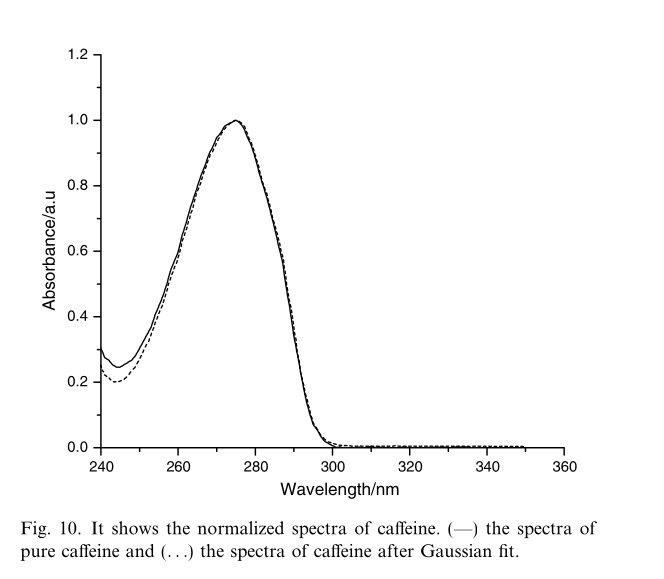
\includegraphics[width=0.8\textwidth]{images/absorbancia_cafeína.png}
	\caption{Resultados con ajuste gaussiano}
	\label{fig:ajuste-gaussiano}
\end{figure} \vspace{0.5cm}

\textbf{Enlace}: \vspace{0.5cm}

\href{https://www.connectedpapers.com/main/5135ae6a3d92e94d6bc22e4c8575d759a8763676/Measurement-of-caffeine-in-coffee-beans-with-UV%2Fvis-spectrometer/graph}{connectedpapers} \vspace{0.5cm}

\href{https://doi.org/10.1016/j.foodchem.2007.10.024}{DOI} \vspace{0.5cm}


\subsubsection{\textbf{Artículo 3:} \textcolor{Sun}{\textbf{Spectrophotometric analysis of caffeine}}} \vspace{0.5cm}

\textbf{Autores}: \textit{Misto}; \textit{Alawiyah}, K.; \textit{Rohman}, L.; \textit{Supriyadi}; \textit{Mutmainnah}; \textit{Purwandari}, E. \vspace{0.5cm}

\textbf{Resumen}: El estudio presenta un método cuantitativo de análisis espectrofotométrico de cafeína, con resultados que validan su precisión y aplicabilidad en diferentes muestras de café. \vspace{0.5cm}

\textbf{Resultados}: \vspace{0.5cm}

\textbf{Enlace}: \href{https://doi.org/xxxxxx}{DOI/Journal link} \vspace{0.5cm}

\subsubsection{\textbf{Artículo 4:} \textcolor{Pesto}{\textbf{Metabolomics fingerprint of coffee species determined (Food Chemistry, 2018)}}} \vspace{0.5cm}

\textbf{Autores}: \textit{Souard}, Florence; \textit{Delporte}, C\'edric; \textit{Stoffelen}, Piet; \textit{Th\'evenot}, {\'E}tienne A.; \textit{Noret}, Nausicaa; \textit{Dauvergne}, Bastien; \textit{Kauffmann}, Jean-Michel; \textit{Van Antwerpen}, Pierre; \textit{St\'evigny}, Caroline. \vspace{0.5cm}


\textbf{Resumen}:Se utilizaron técnicas de huella metabolómica para diferenciar especies de café, lo que facilita la caracterización de cafés de distintas regiones y sus propiedades químicas. \vspace{0.5cm}
\textbf{Resultados}: \vspace{0.5cm}

\textbf{Resultados}: \vspace{0.5cm}


\textbf{Enlace}: \href{https://doi.org/xxxxxx}{DOI/Journal link} \vspace{0.5cm}

\subsubsection{\textbf{Artículo 5:} \textcolor{blue-violet}{\textbf{Degradation kinetics of caffeine in water by UV (2020, Desalination and Water)}}} \vspace{0.5cm}

\textbf{Autores}: \textit{Yisak}, Hagos; \textit{Redi-Abshiro}, Mesfin; \textit{Chandravanshi}, Bhagwan Singh. \vspace{0.5cm}


\textbf{Resumen}El artículo estudia la degradación de cafeína bajo radiación UV, aportando datos útiles sobre su estabilidad y posibles aplicaciones en procesos de tratamiento. \vspace{0.5cm}

\textbf{Resultados}: \vspace{0.5cm}

\textbf{Resultados}: \vspace{0.5cm}

\textbf{Enlace}: \href{https://doi.org/xxxxxx}{DOI/Journal link} \vspace{0.5cm}

\subsection{Vídeo de las búsquedas en las bases de datos}\vspace{0.5cm}

\href{Enlace del vídeo}{Enlace del vídeo}





\end{document}